\def\col{blue}
\documentclass[14pt, \col, hyperref={pdfpagelabels=false}]{beamer}
\usepackage[frenchb]{babel} % langue francaise
\usepackage[utf8]{inputenc} % encodage UTF-8
\usepackage[T1]{fontenc} % encodage de la police de caracteres
\usepackage{lmodern}
\usepackage{listings}
\usepackage{multicol}
\usepackage{pifont} %\ding{number}, 
\usepackage{subfigure}
\usepackage{graphicx}
\usepackage{listings}

\usetheme{Warsaw}
\usepackage[\col]{optional} %red blue green
%% THÈMES couleur
%% \usecolortheme{dolphin}
%% \usecolortheme{seahorse}
%% * thèmes globaux : beetle, crane, fly, seagull.
%% * thèmes internes : lily (enlève surtout des couleurs), orchid, rose.
%% * thèmes externes : whale, seahorse, dolphin

% rubber: rules ./rules.ini

 
\mode<presentation>
{
  %%%% Couleurs
  \definecolor{red2}{rgb}{0.8,0.15,0.15}
  \definecolor{bx}{rgb}{0.45,0.05,0.05}  
  \definecolor{ivoire}{rgb}{1, 0.97, 0.9}
 
  \definecolor{bleu2}{rgb}{0.9, 0.90, 1}
  \definecolor{bleu3}{rgb}{0.15,0.15,0.7}
  \definecolor{myblue}{rgb}{0.50,0.55, 0.8}  
  \definecolor{myblue2}{rgb}{0.25,0.3, 0.65}  
  
 \definecolor{mygreen2}{rgb}{0.15,0.60,0.15}
 \definecolor{green2}{rgb}{0.15,0.40,0.15}
  \definecolor{mygreen}{rgb}{0.40,0.7, 0.4}  
%  \definecolor{lightgreen}{rgb}{0.5,0.8, 0.5}  
  \definecolor{lightgreen}{rgb}{0.95, 1, 98}
  
  \definecolor{medium-grey}{gray}{0.45}
  \definecolor{light-grey}{gray}{0.85}
  
  % Couleur des structures et fond dégradé
  % defaut: green
  \setbeamercolor{normal text}{fg=black,bg=lightgreen}
  \setbeamercolor{structure}{fg=green2, bg=light-grey} 
  \setbeamercolor{alerted text}{fg=green2}
  \setbeamertemplate{background canvas}[vertical
    shading][top=lightgreen!100,bottom=lightgreen!30]
  
  \opt{blue}{
    \setbeamercolor{normal text}{fg=black,bg=bleu2}
    \setbeamercolor{structure}{fg=myblue, bg=light-grey} 
    \setbeamercolor{alerted text}{fg=myblue2}
    \setbeamertemplate{background canvas}[vertical
      shading][top=bleu2!100,bottom=bleu2!30]
  }
  \opt{red}{
    \setbeamercolor{normal text}{fg=black,bg=ivoire}
    \setbeamercolor{structure}{fg=bx, bg=light-grey} 
    \setbeamercolor{alerted text}{fg=red2}
    \setbeamertemplate{background canvas}[vertical
      shading][top=ivoire!40,bottom=ivoire!100]
  }
  \opt{green}{
    \definecolor{green2}{rgb}{0.1,0.60,0.1}
    \usecolortheme{dolphin}
  }   
  
  
  \setbeamertemplate{navigation symbols}{}
  \setbeamerfont{title in head/foot}{size=\scriptsize}
  \setbeamerfont{date in head/foot}{size=\scriptsize} 
  
  % Pied de page
  \setbeamertemplate{footline}{
    \hbox{%
      \begin{beamercolorbox}[wd=.4\paperwidth,ht=3ex,dp=1ex,center]{title in head/foot}
        \usebeamerfont{title in head/foot}\enseignement\hspace{1cm} %\shorttitle
      \end{beamercolorbox}%
      \begin{beamercolorbox}[wd=.5\paperwidth,ht=3ex,dp=1ex,left]{date in head/foot}%
        \usebeamerfont{title in head/foot} 
        \hspace*{1ex} 
        \insertshorttitle
      \end{beamercolorbox}% 
      \begin{beamercolorbox}[wd=.1\paperwidth,ht=3ex,dp=1ex,left]{date in head/foot}%
        \usebeamerfont{date in head/foot} 
        \insertframenumber{} / \inserttotalframenumber%\hspace*{2ex} 
    \end{beamercolorbox}}%
    \vskip0pt%
  }

    % Haut de page
  \setbeamertemplate{headline}{%
    \leavevmode
    \begin{beamercolorbox}[wd=.5\paperwidth,ht=3ex,dp=1.125ex,leftskip=.3cm
        plus1fill,rightskip=.3cm]{section in head/foot}%
      \scriptsize{\insertsection}
    \end{beamercolorbox}%
    \begin{beamercolorbox}[wd=.5\paperwidth,ht=3ex,dp=1.125ex,leftskip=.3cm,rightskip=.3cm
        plus1fil]{subsection in head/foot}%
      \scriptsize{\insertsubsection}
    \end{beamercolorbox}%
  }
  \addtobeamertemplate{headline}{}{%
    \vskip-0.1pt
    \pgfuseshading{beamer@topshade}
    \vskip-2pt}
   %% \let\Tiny=\tiny
  %% \let\TINY=\tiny
}

%% Annonce de plan a chaque transition.
%% \AtBeginSection[]{
%%   \begin{frame}<beamer>
%%     \frametitle{Plan}
%%     \tableofcontents[currentsection,currentsubsection]
%%   \end{frame}
%% }



\newcommand{\bashlisting}[0]{\scriptsize\lstset{language=bash,numbers=left,numberstyle=\tiny,
    xrightmargin=1mm, xleftmargin=1mm, keywordstyle=\color{green2}, %
    keywordstyle[1]=\color{blue}, %
    keywordstyle[2]=\color{yellow}, %
    keywordstyle[3]=\color{red2}}}

\newcommand{\filelisting}[0]{\small\lstset{language=,numbers=left,numberstyle=\tiny,
    xrightmargin=4mm, xleftmargin=6mm, frame=single}}

\definecolor{orange}{rgb}{0.9,0.6,0.4}

\newcommand{\clisting}[0]{\scriptsize
  \lstset{language=c, 
    inputencoding=utf8,
    %identifierstyle=\color{blue},%
    keywordstyle=\color{green2}, %
    keywordstyle[1]=\color{blue}, %
    keywordstyle[2]=\color{yellow}, %
    keywordstyle[3]=\color{red2}, %
    stringstyle=\color{orange}, %
    commentstyle=\color{red2}, %
    numbers=left,
    numberstyle=\tiny,
    xleftmargin=1mm,
    breaklines=true,
}}



\newcommand{\cmd}[1]{\texttt{\footnotesize\textcolor{medium-grey}{#1}}}

\newcommand{\cmdlist}[1]{
  \begin{semiverbatim}\begin{minipage}{\linewidth}  
      \footnotesize\textcolor{medium-grey}{#1}\end{minipage}
\end{semiverbatim}}


\newcommand{\coeur}{c\oe ur\xspace}
\newcommand{\oeuvre}{\oe uvre\xspace}
\newcommand{\coeurs}{c\oe urs\xspace}
\newcommand{\mc}{multic\oe ur\xspace}
\newcommand{\mcs}{multic\oe urs\xspace}

\usepackage{multicol}

%%%%%%%%%%%%%
\def\enseignement{ASR2 Système}
\title[]{\enseignement\\
Notions de virtualisation}
\author{Stéphanie Moreaud}
\institute{Département d'informatique\\
  IUT Bordeaux 1}
\date{}

%%%%%%%%%%%% 
   
\newcommand{\TITRE}[1]{
  \begin{frame} \begin{center}\huge{#1}\end{center}
\end{frame}
}
\newcommand{\FIGURE}[2]{
  \begin{frame} \frametitle{\insertsubsection} 
    \begin{figure} \includegraphics[width=0.8\linewidth]{fichiers-images/#1} 
    \end{figure} 
    \begin{center}\large{#2}\end{center}
\end{frame} }

%%%%%%%%%%%%%%%%%%%%%%%%%%%%%%%%%%%%%
\begin{document}
\begin{frame}
  \titlepage
\end{frame}

\begin{frame}<beamer>
  \frametitle{Plan} 
      \tableofcontents[sections={1-5},currentsection, hideothersubsections] 
\end{frame}
%Annonce de plan a chaque transition.
\AtBeginSection[]{
  \begin{frame}<beamer> \frametitle{Plan}
    \tableofcontents[currentsection, hideothersubsections] 
  \end{frame}
}

\begin{frame}
\frametitle{Bibliographie}
\bibliographystyle{fr-plain}
\small
\nocite{*}    
\bibliography{bib} 
\vspace{0.5cm}    
\end{frame}
%%%%%%%%%%%%%%%%%%%%%%%%%
%%%%%% Let's go!  %%%%%%
%%%%%%%%%%%%%%%%%%%%%%%%%

\section{Principe}
\begin{frame}
\frametitle{\insertsection}
\alert{Virtualisation}~: faire fonctionner sur un seul ordinateur plusieurs systèmes
d'exploitation comme s'ils fonctionnaient sur des ordinateurs distincts. \\
\vspace{0.5cm}
\pause
Pourquoi se serait compliqué? \\
\pause
\vspace{0.5cm}
\underline{Rappel}:
Système d’exploitation en charge de gérer l'ensemble des ressources
matérielles de l’ordinateur (CPU, mémoire vive, périphériques, etc.)
\begin{itemize}
\item[\ding{212}] conçu pour être l'unique administrateur des ressources
\end{itemize}
\vspace{0.5cm}
\end{frame}

\begin{frame}
\frametitle{Notions}
Machine Virtuelle
\begin{itemize}
\item abstraction de la machine physique simulée par un logiciel de virtualisation et
  disposant de son propre OS et environnement d'exécution.
\end{itemize}
\vspace{0.5cm}
Système d'exploitation hôte 
\begin{itemize}
\item OS principal, installé directement sur le matériel 
\end{itemize}
\vspace{0.5cm}
Systèmes d'exploitations \emph{invités} ou \emph{virtualisés}
\begin{itemize}
\item tourne sur la machine virtuelle
\end{itemize}
\end{frame}

\begin{frame}
\frametitle{\insertsection}
OS hôte installé sur l'ordinateur\\
\vspace{0.2cm}
Logiciel de virtualisation, \alert{hyperviseur}
\begin{itemize}
\item crée des machines virtuelles
\item[\ding{212}] environnements clos, isolés, ressources précises
\end{itemize}
\vspace{0.2cm}
OS invités installées sur les machines virtuelles  
\begin{itemize}
\item instances totalement isolées du système hôte et des autres systèmes invités
\end{itemize}
\vspace{0.5cm}

\alert{Virtualisation}: fonctionnement d'OS invités dans 
des machines virtuelles au-dessus d'un OS hôte.
\end{frame}

\section{Intérêts de la virtualisation}
\begin{frame}
  \frametitle{\insertsection ~1/2}
  Regrouper des serveurs sur une même machine
  \begin{itemize}
  \item économie de ressources, d'espace, d'énergie, etc. 
  \item isolation des serveurs
    \begin{itemize}
    \item  si l'un d'eux crash, pas d'effet sur les autres
    \item reboot indépendant 
    \end{itemize}
  \end{itemize}
  \vspace{0.5cm}

  Exécuter plusieurs OS en même temps
  \begin{itemize}
  \item faire une présentation PowerPoint sous Windows et coder sous Linux
  \item vérifier la portabilité d'un logiciel
  \end{itemize}
\end{frame}

\begin{frame}
\frametitle{\insertsection ~2/2}
  Pérennité de vielles applications 
  \begin{itemize}
  \item possibilité de faire tourner les applications sur de ``vieux'' OS
  \end{itemize}
  \vspace{0.5cm}
  Facilité de déploiement pour les utilisateurs
  \begin{itemize}
  \item utilisation d'images systèmes, migration de machines,
  \item pas de modification de l'installation   
  \end{itemize}
  \vspace{0.5cm}
  Gestion transparente de périphériques
  \begin{itemize}
  \item exportation d'un OS à l'autre
  \end{itemize}
\end{frame}


\section{Différents types de virtualisation}
\subsection{Émulation}
\begin{frame}
\frametitle{\insertsubsection}
Environnement expose du matériel virtuel 
\begin{itemize}
\item processeur, mémoire, disque, réseau, ...
\item entièrement simulé  
\end{itemize}

OS invité communique avec matériel simulé
\begin{itemize}
\item au travers de pilotes
\item instructions transmises à l’hyperviseur
\item[\ding{212}] hyperviseur fait appel à l'OS pour les exécuter.
\end{itemize}
\vspace{0.5cm}
\ding{212} Fonctionne avec n'importe quel OS invité qui supporte le matériel virtuel\\
\ding{212} Très lent\\
\vspace{0.2cm}
Ex: qemu
\end{frame}


\begin{frame}
\frametitle{\insertsubsection}
\vspace{-0.5cm}
\begin{figure}
  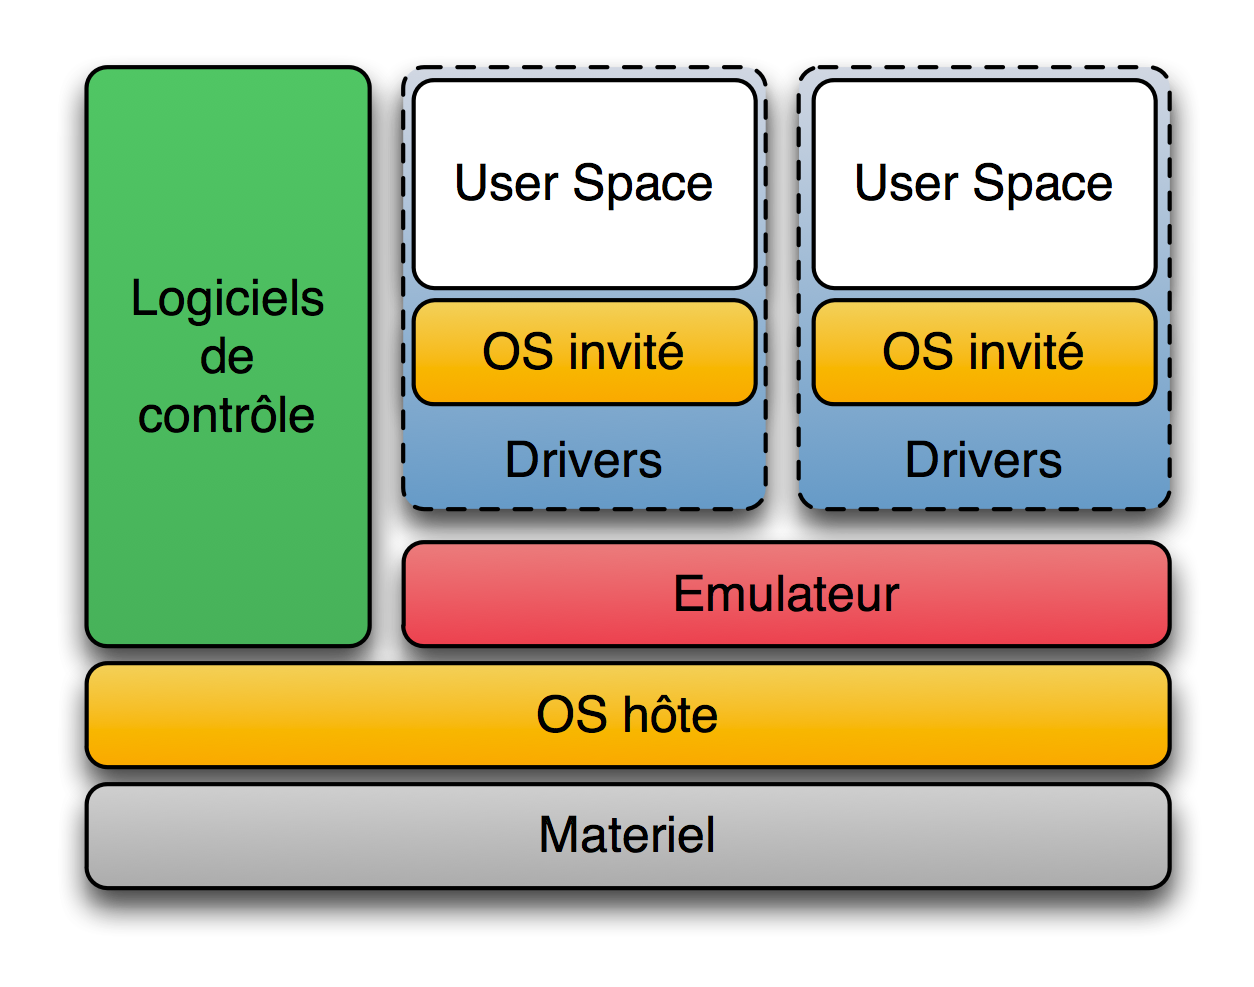
\includegraphics[width=0.8\linewidth]{fig4/Diagramme_ArchiEmulateur.png}
\end{figure}
\vspace{-0.5cm}
\small{source~: \href{http://fr.wikipedia.org/wiki/Fichier:Diagramme_ArchiEmulateur.png}{\textcolor{blue}{Wikipedia}}}
\end{frame}


\subsection{Virtualisation totale}
\begin{frame}
\frametitle{\insertsubsection}
Émulation plus restrictive 
\begin{itemize}
\item processeur de la machine virtuelle du même type que celui de la
  machine physique
\end{itemize}
\vspace{0.5cm}
Hyperviseur peut être placé au niveau de l'OS
\begin{itemize}
\item accès au matériel via les pilotes de l'OS hôte
\end{itemize}
\vspace{0.5cm}
\ding{212} meilleures performances que l'émulation\\
\vspace{0.2cm}
Ex: VMWare, VirtualPC
\end{frame}

\subsection{Paravirtualisation}
\begin{frame}
\frametitle{\insertsubsection}
Hyperviseur = OS très simple
\begin{itemize}
\item tourne sur le matériel 
\item partage le matériel entre plusieurs OS invités
\item exécute les instructions privilégiées 
\end{itemize}
\vspace{0.2cm}
Un OS maître
\begin{itemize}
\item hyperviseur lui confie les périphériques 
\item les exporte aux autres OS
\end{itemize}
\vspace{0.5cm}
\ding{212} meilleures performances\\
\ding{212} OS invités modifiés pour parler à l'hyperviseur\\
\vspace{0.2cm} Ex: Xen
\end{frame}

\begin{frame}
\frametitle{\insertsubsection}
\vspace{-0.5cm}
\begin{figure}
  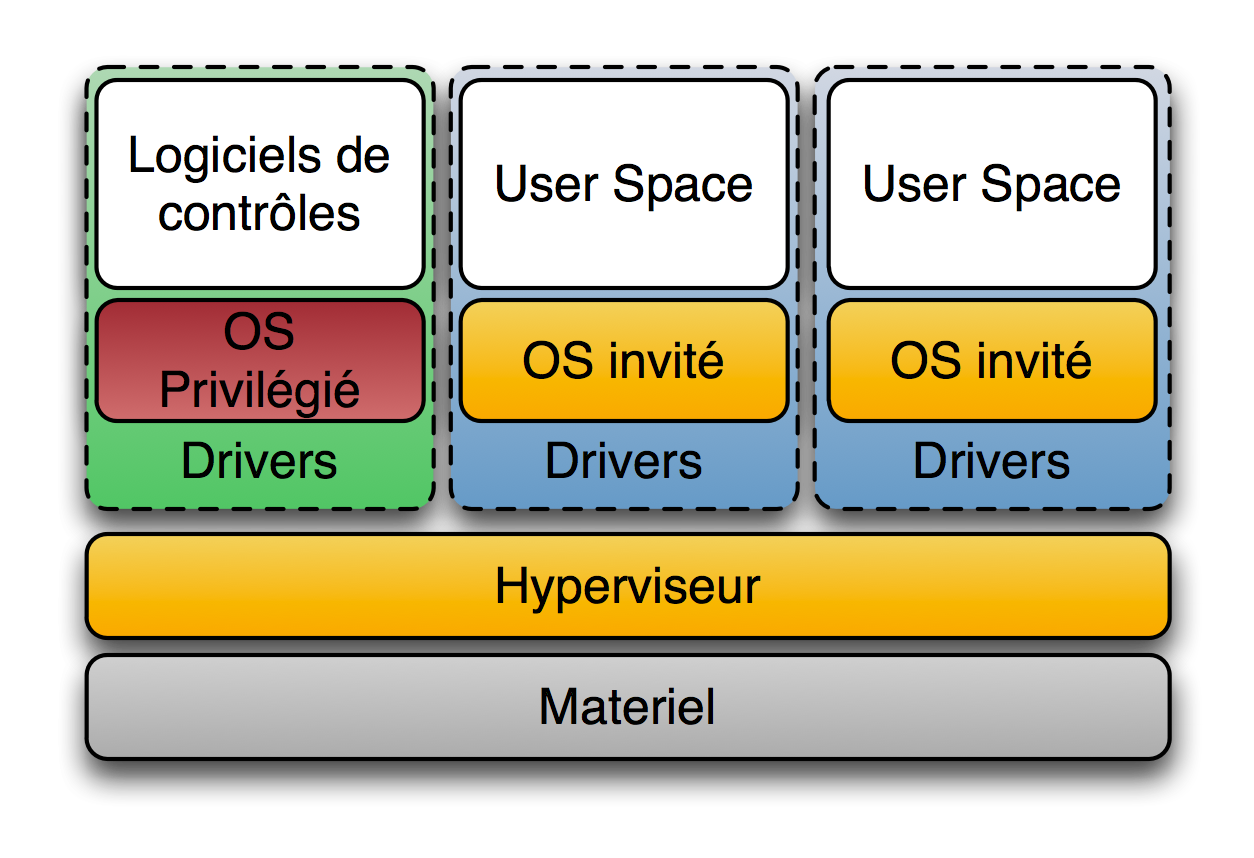
\includegraphics[width=0.9\linewidth]{fig4/Diagramme_ArchiHyperviseur.png}
\end{figure}
\vspace{-0.5cm}
\small{source~: \href{http://fr.wikipedia.org/wiki/Fichier:Diagramme_ArchiHyperviseur.png}{\textcolor{blue}{Wikipedia}}}
\end{frame}


\subsection{Virtualisation matérielle}
\begin{frame}
\frametitle{\insertsubsection}
Instructions ajoutés au processeur pour qu’il serve d’hyperviseur
\begin{itemize}
\item OS invités au même niveau que l'OS hôte
\item pas d'émulation du processeur
\item pas de modification des OS
\end{itemize}
\vspace{0.5cm}

\ding{212} performances optimales \\
\ding{212} nécessite un processeur spécifique
\end{frame}
\end{document}

% LocalWords:  blue ASR width fichiers-images beamer currentsection Let's d'OS
% LocalWords:  hideothersubsections hyperviseur reboot PowerPoint Windows l'OS
% LocalWords:  qemu Wikipedia VMWare VirtualPC Paravirtualisation Xen
